\section{Optimizaciones}

Aqu\'{i} van las optimizaciones.

Peque\~{n}a ayuda (mirar optimizaciones.tex para ver el c\'{o}digo):

Como poner una lista de elementos:
\begin{itemize}
   \item Elemento 1
   \item Elemento 2
\end{itemize}

Como poner una figura:
\begin{figure}[ht]
   \centering
   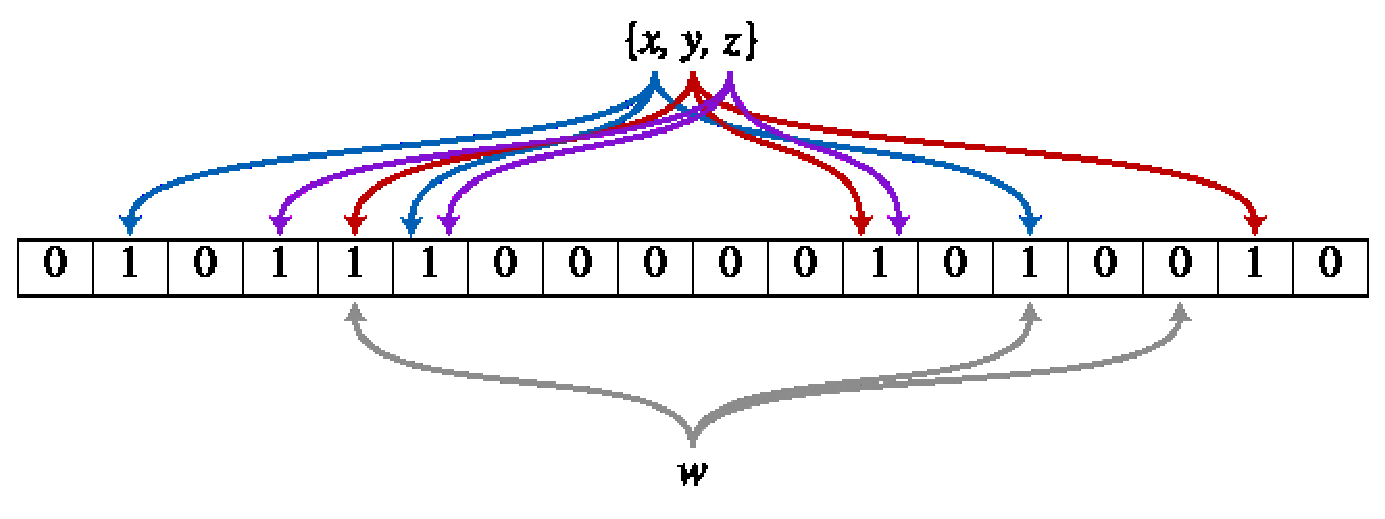
\includegraphics[keepaspectratio=true,width=.6\textwidth]{figures/muestra}
\end{figure}

Como poner una tabla:
\begin{center}
   \begin{tabular}{| c || c | c | c |}
      \hline
      	           & Load	& Store		& Total		\\ \hline \hline
	Accesses   & 105353	& 21423		& 126776	\\ \hline
	Hits       &  11644	&  1837		&  13481	\\ \hline
	Misses     &  93709 	& 19586		& 113295	\\ \hline
	Miss rate  & 88.95\%	& 91.43\%	& 89.37\%	\\ \hline
   \end{tabular}
\end{center}

Como poner c\'{o}digo:
\begin{verbatim}
POS1 = vector[hash_function_1(value)];
POS2 = vector[hash_function_2(value)];
if (POS1 == 0 || POS2 == 0) return FALSE;
return TRUE;
\end{verbatim}

% vim: filetype=tex tw=75
